
\documentclass[letterpaper,twocolumn,10pt]{article}
\usepackage{usenix2019_v3}
\usepackage{algorithmic}
\usepackage{algorithm}
\usepackage{listings}
\usepackage{pifont}
\usepackage{multirow}
\usepackage{graphicx}
\usepackage{caption}
\usepackage{xcolor}
\usepackage{booktabs}

% to be able to draw some self-contained figs
\usepackage{tikz}
\usepackage{amsmath}
\usepackage{cleveref}
\crefname{section}{§}{§§}
\Crefname{section}{§}{§§}

% new commands
\newcommand{\name}{CATFlow}

%-------------------------------------------------------------------------------
\begin{document}
%-------------------------------------------------------------------------------

%don't want date printed
\date{}

% make title bold and 14 pt font (Latex default is non-bold, 16 pt)
\title{\Large \bf \name{}: Data-Monistic Parallelization Plan Discovery for Distributed Training}

%for single author (just remove % characters)
\author{
% {\rm Your N.\ Here}\\
% Your Institution
% \and
% {\rm Second Name}\\
% Second Institution
% % copy the following lines to add more authors
% % \and
% % {\rm Name}\\
% %Name Institution
} % end author

\maketitle

%-------------------------------------------------------------------------------
\begin{abstract}
%-------------------------------------------------------------------------------
As neural networks grow in size and complexity, distributed training across multiple devices becomes essential. Yet, finding an efficient parallelization plan is difficult due to the vast search space, which includes both strategy choices and parameter settings for each strategy. Most existing methods search parameters within a fixed strategy space like 3D parallelism, while recent work enables experts to manually construct custom strategy spaces. However, both approaches suffer from two key limitations: they either have rigid strategy spaces or lack completeness in strategy definition, and they are limited to performing automated search within a fixed strategy. These limitations make it difficult to discover efficient parallelization strategies beyond existing human designs.

To address this, we introduce \name{}, a training parallelization plan generation framework that presents a key insight: defining a strategy space with a purely \textbf{data-centric} perspective (focusing on data trajectory) offers greater expressiveness, completeness, and search tractability compared to operator-centric approaches (focusing on operator scheduling). \name{} describes parallelization strategies using three fundamental representation entities: tensors, space-time coordinates, and their relationships formalized as constraints. \name{} introduces a set of primitives for constructing and manipulating these abstractions, which demonstrates greater expressiveness, covering operator schedulings like 3D parallelism, co-optimizations of computation and data movement like FSDP, and dataflow-driven strategies like WeiPipe—capabilities that extend beyond existing frameworks.

Leveraging these unified data-centric abstractions, we propose a constraint-based potential descent algorithm for parallelization strategy search. This enables the \textbf{automatic discovery} of \textbf{novel parallelization strategies}. Using \name{}, we discover a new strategy, ZERO-4, which simultaneously achieves the low memory consumption of ZERO-3 and performance approaching that of ZERO-2. Furthermore, \name{} delivers an XX\% performance improvement in resource-constrained scenarios through coordinated two-level strategy and parameter optimizations.
% 可能最终不会采用two-level strategy and parameter optimizations这种说法
\end{abstract}

\section{Introduction}
\label{sec:intro}

% 明确一下名词
% strategy space -> strategy -> plan. Strategy space包含了多个strategy
% 而plan是一个具体的并行实现方式。对于传统的方法，确定了一个strategy的参数之后，就会得到一个plan
% 本文的路径 strategy space -> strategy 与传统路径是有一定冲突的，所以我们将传统路径描述为stategy template -> plan
% 不要说implementation，implementation是指我们系统的工程实现方式。比如说用的Python构建接口啊等等
% 另一个小问题：operators准确的说是不是computation及其相关的storage -> 是的
Deep Neural Networks (DNNs), particularly large language models (LLMs), have achieved advanced performance across a wide range of domains. However, the efficient training of large-scale models necessitates substantial resources, frequently surpassing the capabilities of a single device~\cite{narayanan2021efficient}. Consequently, distributing training across multiple devices is crucial. The core challenge lies in identifying an efficient parallelization plan for distributed training. An NN model can be formally modeled as a dataflow graph~\cite{lin2023songc}, where nodes represent either data storage (tensors) or computations (operators), and directed edges represent dependencies between nodes. A comprehensive parallelization strategy specifies the distribution and scheduling of storage and computation in both space (device placement) and time (execution order)~\cite{qiu2025moirai, huang2019yugong, lin2024nnscaler}. The space of feasible parallelization plans is vast, and the problem of determining an optimal plan is NP-hard~\cite{liu2024aceso}.

Due to the immense search space and complex constraints, distributed training optimizations often rely on meticulously designed strategies that incorporate domain expertise. Examples include Megatron-LM~\cite{shoeybi2019megatron, narayanan2021efficient}, which incorporates parameterized parallelization strategies known as data, tensor, and pipeline parallelism (DP, TP, PP, collectively termed 3D parallelism) to support Transformer-based models, and Piper~\cite{tarnawski2021piper} and Alpa~\cite{zheng2022alpa}, which organize parallelization choices into a two-level hierarchical space termed staged single-program, multiple-data (SPMD). In this approach, the system first searches for a plan based on pipeline (inter-operator) parallelism and then on tensor (intra-operator) parallelism within each pipeline stage. These approaches typically first define a space that is a combination of existing strategies and subsequently perform a parameter search within its configurations.

\begin{table*}[t!]
\small
\centering
\setlength{\tabcolsep}{4pt}
\caption{High-level comparison of paradigms.}
\label{tab:landscape}
\begin{tabular}{p{0.14\linewidth}p{0.26\linewidth}p{0.26\linewidth}p{0.26\linewidth}}
\toprule
\textbf{Feature} & \textbf{Classical} (e.g., Megatron-LM) & \textbf{nnScaler} & \textbf{\name{}} \\
\midrule
\textbf{Fundamental view} & \textbf{Strategy-centric:} fixed library of named strategies (e.g., DP, PP, TP) & \textbf{Operator-centric:} define strategy by operator behaviors & \textbf{Data-monistic:} define strategy by data trajectories \\
\textbf{Space definition / Prim. semantics} & \textbf{Fixed templates:} combination of existing strategies (e.g., 1F1B, 3D) & \textbf{Constructive:} default-deny, explicitly permit; build form zero. & \textbf{Subtractive:} default-allow, explicitly forbid; carve from universal set\\
\textbf{Completeness} & \textbf{Low:} combination of built-ins & \textbf{Medium:} complete for computation scheduling & \textbf{High:} covering computation, storage, and communication co-optimization \\
\textbf{Expressiveness} & \textbf{Low:} combination rules of built-ins & \textbf{Medium:} custom operator schedules, no data-centric optimizations. & \textbf{High:} fine-grained control over tensor life-cycle and events \\
\textbf{Searchability} & \textbf{Parameter search} & \textbf{Para. search in user-defined space} & \textbf{Automatic strategy discovery} \\
\textbf{Dataflow handling} & Implicit and fixed by chosen strategy & Implicit side-effect of operator & Explicit and first-class target \\
\bottomrule
\end{tabular}
\end{table*}

While many studies~\cite{tarnawski2021piper, zheng2022alpa, liu2024aceso} focus on specific plan searches within different strategy classes, recent work~\cite{lin2024nnscaler} advocates domain-specific primitives that allow experts to construct customized strategies. This paradigm recognizes that variations in hardware, workload characteristics, and expert knowledge can lead to distinct preferred strategies, thus providing a more flexible framework to unlock further optimization opportunities. Experts define novel strategies with their designed patterns and search configurations.

However, existing approaches still face two limitations. First, they either define rigid strategy spaces or lack completeness in strategy specification, making it hard to capture more potential opportunities. Although nnScaler~\cite{lin2024nnscaler} represents a significant advance in strategy construction—capable of describing most existing training plans and new expert-crafted strategies—it remains unable to express optimizations involving coordinated data movement, such as FSDP~\cite{rajbhandari2020zero} and WeiPipe~\cite{lin2025weipipe}, thus hindering the ability to fully exploit hardware resources. Second, the quality of this pre-designed space is a critical determinant of the achievable performance of these frameworks, which are limited to automated search within a fixed strategy space; search algorithms select among efficient configurations and parameter settings (e.g., partition sizes, device assignments, execution order) rather than enabling the automatic discovery of unforeseen strategies.

For methods that define strategies using domain-specific primitives, their expressiveness is constrained by the underlying abstractions and specifications. Existing approaches are predominantly operator-centric. For instance, nnScaler~\cite{lin2024nnscaler} introduces three primitives—\texttt{op-trans}, \texttt{op-assign}, and \texttt{op-order}—for specifying operator behaviors. These approaches focus on computation and implicitly bind data movement to operator scheduling. We present a core contrary insight: adopting a \textbf{data-monistic} perspective yields a more expressive and complete abstraction for strategy-space construction, in which parallelization plans are defined by describing the trajectory of data and imposing constraints on its movement. From this viewpoint, computation is implicitly represented as a \textbf{constraint} on dataflow; that is, its occurrence means all required data must meet at the same device, and the scheduling of computation can be deduced naturally from the constraints that govern data movement.

Building on this insight, we present \name{}—a framework for describing, generating, and searching for distributed-training plans. Its core is an abstraction centered on a single entity: the constraint-aware tensor (CAT). The constraints associated with each tensor specify its space-time coordinates (when and where a tensor resides). \name{} provides a set of primitives for manipulating CATs to constrain strategies that coordinate data movement and computation and handle complex dependencies such as recomputation.


% \begin{table*}[t]
% \small
% \centering
% \setlength{\tabcolsep}{4pt}
% \caption{High-level comparison of paradigms.}
% \label{tab:landscape}
% \begin{tabular}{llll}
% \toprule
% Feature & Traditional & nnScaler & \name{} \\
% \midrule
% Fundamental view & Strategy-centric & Operator-centric & Data-monistic \\
% Space definition & Fixed templates & Constructive & Declarative \\
% System role & Parameter search & Template search & Strategy discovery \\
% Expressiveness & Low (built-ins) & Medium (op-schedules) & High (data \& op) \\
% Dataflow handling & Implicit & Implicit & Explicit \\
% \bottomrule
% \end{tabular}
% \end{table*}

Unlike pre-designed strategy spaces, \name{} employs declarative, subtractive primitives to carve a \textit{universal} strategy space through constraints. Prior approaches rely on constructive primitives to explicitly specify scheduling behavior, requiring users to design what a policy should be. In contrast, \name{}'s reductive methods allow designers to stipulate what a policy should not be. The resulting strategy space therefore encompasses both established and unforeseen designs, thereby opening opportunities for strategy discovery. Further, the data-monistic perspective provides a unified, continuous landscape that improves optimization tractability and supports smooth transitions between plans during search. Building on these foundations, we propose a constraint-based potential descent algorithm that discovers novel parallelization strategies beyond parameter tuning. Table~\ref{tab:landscape} summarizes the key differences between \name{} and others.

\name{}'s core contributions are summarized as follows:

1. \textbf{Data-Monistic Parallelization Strategy Abstraction and Space Construction:} We introduce \name{}, a framework featuring novel abstractions and primitives for constructing parallelization strategy spaces in distributed NN training. \name{} enables the explicit and complete specification of strategies involving both computation and data movement from a data-monistic view. This stands in contrast to existing operator-centric approaches, unlocking a strictly larger and more expressive strategy space.

2. \textbf{Automatic Discovery of Novel Strategies:} Leveraging \name{}'s unified abstractions, a strategy space can be reductively carved by constraining CATs. Within the strategy space, we propose a hierarchical potential descent algorithm that enables the automatic discovery of unforeseen parallelization strategies, going beyond traditional parameter search within a fixed strategy pattern.

3. \textbf{Presentation of New Strategies:} Based on \name{}, we present new, efficient distributed training strategies for resource-constrained scenarios that match or surpass state-of-the-art, manually designed solutions. These include a novel strategy that achieves the memory efficiency of ZeRO-3 and performance approaching that of ZeRO-2, as well as delivering near-linear scaling and improved hardware utilization.

\section{Background \& Motivation}

\subsection{Search Space for Parallelization Plans}

% 首先说有很大的搜索空间
% 然后介绍了了DP, TP, PP以及3D并行
% 介绍一下Tessel的PP, Megatron的3D并行search space, Alpa和Piper的staged SPMD
% 介绍一下exiting search spaces存在limitations, 这样的predefined的search space是针对固定的workload准备的, 对于更大范围的workload来说，不够通用，会丢掉很多优化机会，比如说AlphaFold2的3F1B和embedding层的low computation utilization问题

A \textit{parallelization plan} specifies how a model is partitioned and scheduled across multiple devices, including the distribution of tensors (data), operators (computations), and their temporal order. The challenge lies in the vast combinatorial space of possible plans, and finding the optimal plan is NP-hard. Most approaches use either handcrafted parallelization plans or constrained search spaces. Common strategies include:

\textit{Data Parallelism:} Replicates operators across devices, partitioning the input batch. Each replica processes a portion of the batch and shares model parameters. \textit{Tensor Parallelism:} Partitions operators and tensors along dimensions beyond the batch, enabling distribution of a single operator across devices—crucial for models exceeding single-device memory. \textit{Pipeline Parallelism:} Divides the model into sequential stages assigned to device meshes and executed in a pipelined fashion. The input batch is split into micro-batches, processed in a scheduled order. These strategies are often combined as \textit{3D Parallelism}. Megatron-LM~\cite{} exemplifies this, combining DP, TP, and PP for Transformer models. Piper and Alpa extend this with staged SPMD, first searching for a PP strategy, then an SPMD plan within each stage (Alpa allows more flexible TP configurations). While effective, these approaches often fix schedules like 1F1B and overlook fine-grained micro-batch scheduling. Tessel addresses this by optimizing micro-batch scheduling given operator placement.

Existing methods define a constrained search space and search within it, so performance depends on the quality of the predefined space, which is often workload-specific. For broader workloads, this can miss optimization opportunities. For example, AlphaFold2 requires three forward passes before one backward pass, which traditional 1F1B scheduling cannot handle. In multilingual models, basic 3D parallelism or staged SPMD may cause large embedding tables to consume many devices, resulting in low computational utilization. These cases show how new optimization opportunities are hard to capture with fixed search spaces.

\subsection{Parallelization Strategy Construction}

% 为了解决上述问题，recent research, especially nnScaler, 希望能够提出一种更灵活的方式来构建parallelization plan space, enable domain experts to find more effective training plans for their models. nnScaler中主要提出了三种primitives: nnScaler introduces \texttt{op-trans}, \texttt{op-assign}, and \texttt{op-order} to specify operator partitioning, spatial placement, and temporal scheduling, respectively. 通过这三种基本的primitives可以定义广阔的并行空间, 再结合nnScaler中所提出的powerful的constraint表示，which can prune the search space defined by primitives, nnScaler可以表示现有工作所不能包含的一系列并行search space，比如特殊的PP strategy for alphafold with 3 forward process and 1 backward, stage_spmd + 特殊的mapping方式for specific ops, like embedding in Language models, 语序不同的PP stage share devices. 

% 但是，尽管nnScaler的强大能力，我们发现他所能够表示的并行搜索空间仍然是有限，因为neglect掉了 the crucial role of data movement and the potential for \textbf{co-optimizing computation and dataflow}. 我们主要关注两类search space that cannot be expressed  by existing works. 首先是standalone dataflow 优化，for example, 在nnScaler中，提出了and so each device holds only one split operator. However, we observe that sometimes multiple split operators can share a single device and compute in a streamlined manner, resulting in fewer devices required for each pipeline stage and less memory consumption. Although the streamlined computing of multiple split operators may slow down the computing process, the reduced communications across fewer devices can lower cost and speed up the overall process. Normally, the streamlined computing的结果应该在本地reduce，但实际上，nnScaler无法限制数据移动的轨迹，如果我在每一次计算过程之后都在不同的device之间去做reduce，显然会引起更大的通信代价，这说明如果我们只关注operator本身的parallelization, 而忽略了dataflow相关的organization以及scheduling的话, 会丢失很多优化的机会，并且也无法准确定义完整的并行行为。

To address the limitations of existing strategy templates, recent research, particularly nnScaler, aims to provide a flexible framework for constructing diverse parallelization strategy templates. nnScaler introduces three core primitives: \texttt{op-trans} (operator partitioning), \texttt{op-assign} (spatial placement), and \texttt{op-order} (temporal scheduling). By combining these primitives with constraints, nnScaler can describe a broader spectrum of parallelization strategy templates than previous approaches, including specialized pipeline schedules (e.g., 3F1B for AlphaFold2) and staged SPMD with customized mappings for operators like large embedding tables. However, these methods for constructing strategy templates typically adopt an operator-centric abstraction, which leads to inherent limitations.

In modern distributed training, performance depends not only on how computation is parallelized but also on how data is orchestrated and moved~\cite{huang2019yugong, qiu2025moirai}. Many state-of-the-art optimizations are explicitly dataflow-driven—e.g., Fully Sharded Data Parallelism (FSDP) \cite{rajbhandari2020zero}, activation recomputation, and offloading—which tightly coordinate parameter sharding, prefetching, asynchronous communication, and conditional transfers with computation scheduling. However, operator-centric frameworks \cite{lin2024nnscaler} treat data movement as an implicit byproduct of operator placement and ordering, lacking mechanisms to explicitly control or co-optimize dataflow; consequently, they cannot express strategies that jointly orchestrate computation and data movement (e.g., FSDP) or manage complex recomputation dependencies. This limitation prevents the discovery and representation of a critical class of high-performance parallelization plans, motivating a more expressive, data-centric abstraction.

% \subsection{Limitations of Operator-Centric Abstractions}

% In modern distributed training, performance is increasingly dictated not just by how computation is parallelized, but by how data is managed and moved~\cite{huang2019yugong, qiu2025moirai}. A growing number of advanced optimizations focus explicitly on dataflow, such as Fully Sharded Data Parallelism (FSDP)~\cite{rajbhandari2020zero}, which coordinates parameter sharding with computation, or sophisticated memory-saving techniques like activation recomputation and offloading. These strategies involve complex data trajectories—prefetching, asynchronous communication, and conditional data movement—that are tightly coupled with the computation scheduling.

% However, existing operator-centric frameworks~\cite{lin2024nnscaler} struggle to express these data-centric optimizations. By treating data movement as an implicit side-effect of operator placement and scheduling, they lack the vocabulary to explicitly control or co-optimize dataflow. For example, nnScaler cannot express optimizations that tightly coordinate computation and data movement, such as FSDP, or complex dependency management in recomputation strategies. This limitation prevents existing systems from discovering or representing a critical class of high-performance parallelization plans, motivating the need for a more expressive, data-centric abstraction.

\section{Abstraction with Constraint-Aware Tensor}
\label{sec:abstraction}

Distributed training requires not only partitioning computation, but also control over data movement and their coordinated scheduling. To address the limitations of operator-centric abstractions, \name{} introduces a unified entity: the \textbf{constraint-aware tensor (CAT)}, which is associated with three tightly coupled concepts: \textit{Tensor}, \textit{Space-Time Coordinate}, and \textit{Constraint}. 
% 之所以不在此处区分强约束与弱约束，是因为CATFlow的核心目标在于帮助用户构建策略空间，而非直接指定具体的并行策略。
% 搜索算法的任务是在该策略空间内寻找最优解，而不是突破或打破这些约束，因此强弱约束的区分在此意义不大。
% 此外，所谓的强约束通常对应于计算相关的约束，其作用与下文所述的Inter-tensor constraint基本一致。

\textit{Tensor}: Represents a data block within the computation graph, including both persistent model parameters and transient intermediate results.

\textit{Space-Time Coordinate}: Denotes the location (device) and temporal position. Rather than using physical time, the temporal coordinate is defined by Lamport logical time~\cite{lamport2019time}, which reflects the execution order (see Section \ref{sec:dependency}).

\textit{Constraint}: Specifies the relationships between tensors and their space-time coordinates, determining where (device/location) and when (temporal order) a tensor exists or is operated upon. This enables explicit modeling of both data placement and execution timing for each tensor instance. Constraints can be further categorized as:

\begin{itemize}
    \item \textbf{Intra-tensor constraint}: Restricts the trajectory of a single tensor across different space-time coordinates, governing its movement and lifecycle.
    \item \textbf{Inter-tensor constraint}: Ensures that multiple tensors coincide at the same space-time coordinate, thereby enabling computation or enforcing dependencies.
\end{itemize}


\begin{figure}[h]
  \centering
  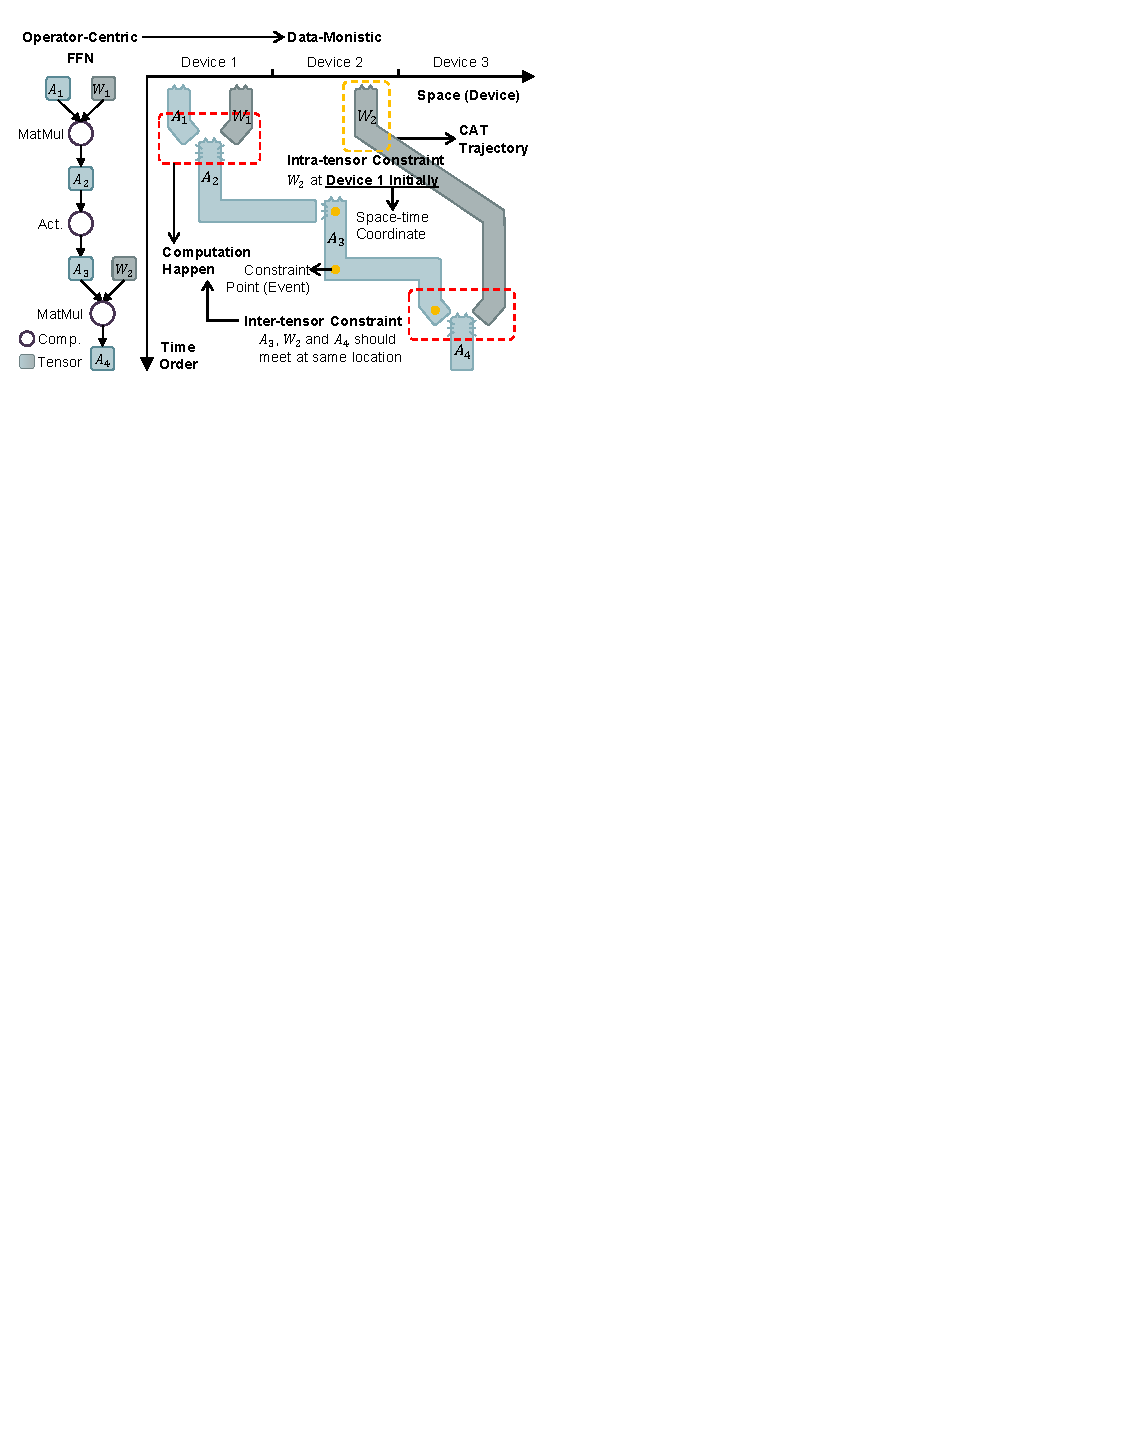
\includegraphics[width=1\linewidth]{figures/abstractions.pdf}
  \caption{Illustration of the data-monistic abstraction using an FFN layer in Transformer as an example. Each tensor is annotated with constraints explicitly with space-time coordinates. This abstraction enables fine-grained control over tensor partitioning, assignment, reduction, ordering, etc., supporting expressive strategies beyond operator-centric approaches.}
  \label{fig:abstractions}
\end{figure}

% Figure \ref{fig:primitives}(a) illustrates the difference between operator-centric and dataflow-centric perspectives. From the dataflow perspective, everything in the graph is represented by the \textit{flow} of data. Each tensor is not merely a static data block in memory, but a dynamic process. The \textit{head} of the arrow in Figure \ref{fig:primitives}(a) represents the beginning of tensor generation, and the \textit{tail} represents the completion of data generation. If the flow of \texttt{tensor1} and the flow of \texttt{tensor2} meet, the generation of \texttt{tensor3} will naturally be triggered. This dataflow perspective for describing NN workloads forms the foundation of our dataflow-centric primitives.


% 在之前的版本中，event 被放在 dependency 那一节介绍，但从逻辑上看，constraint point 应作为完整抽象描述的一部分，应该在此处介绍。
% 但这样做也有一些风险：
% 1. generation 和 consumption event 实际上就代表了计算。如果我们的抽象对其进行了精细描述，实际上等价于直接描述了计算的调度。我们的做法是用一种统一的方式来描述计算与数据流调度的超集。但在文章中不宜直接这样解释，否则会削弱“二元对立”的叙事，影响创新性的判断。
% 2. 末尾的 event 更准确地说代表数据释放，而非消费。
% 3. 在此处介绍 event 机制可能会增加文章前期的阅读难度，使 monistic 抽象显得复杂（而此处又无法展示这种复杂性带来的好处）。但总体来看，这一想法还是比较直接的。
% 4. 不同的 event 蕴含不同的“细节”。例如我们将 move 放在发送方而非接收方，那么如何确定发送目标？可通过下一个 event 的空间坐标判断。另外，约束向量并未描述设备间通信带宽和延迟等信息。
% 5. 关于 move 实现的一个潜在冲突：有时我们不希望指定两个约束点之间的具体路径（留给搜索算法探索），即两个约束点之间搜索算法可以插入新的约束点。这种“路径未知性”可能与 move 默认发送到下一个约束点所在设备的语义存在一定冲突。

A CAT is more than a static data block—it encapsulates both the data itself and the dynamic trajectory of its generation/initiation, movement, and release. We use a series of \textbf{constraint points} to better describe the space-time trajectory of a CAT. These points form a \textbf{constraint vector}, which expresses the different space-time positions of a CAT during training. In the implementation, these constraint points are realized as \textbf{events} that operate on the tensor. For instance, the first and last points in the constraint vector typically represent the CAT's generation and release events, respectively, and intermediate points typically signify movement events between devices. Figure \ref{fig:abstractions} demonstrates how a simple FFN computation is represented in the CAT abstraction. For example, the trajectory of tensor $A_3$ is represented by the following constraint vector: $\mathbf{C}_{A_3} = [(\rm{Device}_2, t_1), (\rm{Device}_2, t_2), (\rm{Device}_3, t_3)]$.
$\mathbf{C}_{A_3}$ specifies its lifecycle: generated on Device 2 from consuming $A_2$, then sent to Device 3, where it is consumed to produce $A_4$.

This data-monistic abstraction is strictly more expressive than operator-centric approaches. Instead of treating data movement as an implicit side-effect of operator scheduling, \name{} defines computation as a consequence of data colocation: an operator executes when its input tensors meet at the same space-time coordinate. By describing the trajectory of data, we uniformly define the scheduling of computation, storage, and communication. This reversal allows \name{} to represent any operator-centric plan, plus a wider range of strategies that co-optimize computation and dataflow or manage complex data dependencies.

\section{Primitives for Abstraction Manipulation}
\label{sec:primitives}

While directly manipulating each tensor's fine-grained constraints offers maximum flexibility, doing so for a complete parallelization plan is both tedious and error-prone. To simplify the construction of data-monistic abstractions, \name{} provides six high-level primitives. These primitives serve as auxiliary tools for building strategy spaces, connecting tensors and space-time coordinates through constraints to generate valid representations within \name{}. They can be categorized into three groups:

\textbf{Tensor distribution primitives}: This group, including \texttt{split}, \texttt{assign}, \texttt{copy}, and \texttt{reduce}, manages the spatial distribution of tensors. They collectively define how data is partitioned, placed, and moved across devices.

\textbf{Dependency management primitives}: This group, comprising \texttt{order} and \texttt{redirect}, governs the logical temporal orders between events. \texttt{order} enforces a specific execution sequence between events, while \texttt{redirect} transfers and creates dependencies across tensors.

\textbf{Strategy space delineation}: This mechanism is used to declaratively define and constrain the search space. For instance, a \texttt{domain} specifies the permissible range of values for a given primitive's configuration (e.g., space-time coordinates), thereby defining the boundaries of the search space.

In the following sections, we will demonstrate their usage through a walkthrough example.

\subsection{Walkthrough Example}

FSDP is a widely-adopted data parallelism strategy that coordinates computation and data movement. It shards model parameters, gradients, and optimizer states across devices to reduce memory. During training, each device holds only a shard of the weights. For a forward pass, a device gathers the full parameters for the current layer, performs the computation, and then discards the full parameters, keeping only its shard. For the backward pass, gradients are computed locally and then reduced and sharded directly to the target devices using a reduce-scatter operation, avoiding redundant storage. This sharding strategy is often described in levels, inspired by the ZeRO (Zero Redundancy Optimizer) framework~\cite{rajbhandari2020zero}. ZeRO-1 shards optimizer states, ZeRO-2 adds gradient sharding, and ZeRO-3 (the typical FSDP implementation) shards parameters as well for maximum memory savings. Algorithm \ref{alg:fsdp} shows how \name{}'s primitives can represent the core of ZeRO-2/3. 

\begin{figure}[h]
  \centering
  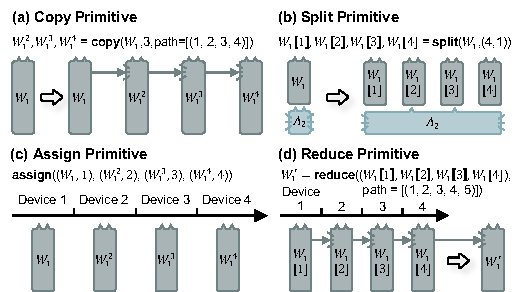
\includegraphics[width=1\linewidth]{figures/primitive_intro1.pdf}
  \caption{Illustration of data-centric primitives. (a) The \texttt{copy} primitive replicates tensors, enabling data replication across devices. (b) The \texttt{split} primitive partitions tensors, implicitly defining operator partitioning. (c) The \texttt{assign} primitive assigns tensors to devices, implicitly defining operator placement. (d) The \texttt{reduce} primitive manages data movement.}
    \label{fig:primitive_intro1}
\end{figure}

\begin{algorithm}[h]
\caption{Primitive program for FSDP (ZeRO-2 \& 3). The \texttt{weight} tensor is either replicated (ZeRO-2) or sharded (ZeRO-3), while gradients and optimizer states are sharded. Assume the number of devices is 4.}
\label{alg:fsdp}
\begin{algorithmic}[1]
\STATE \# ZeRO-2: Replicate weights
\STATE $weight^2$, $weight^3$, $weight^4$ = \textbf{copy}($weight$, 3)
\STATE \# Or ZeRO-3: Shard weights
\STATE $weight[1$ to $4]$ = \textbf{split}($weight$, 4)
\STATE \textbf{assign}($weight^i$ or $weight[i]$, $device_i$) \#$weight^1$ is $weight$
\STATE \# Shard gradients of weights
\STATE $gradient[1$ to $4]$ = \textbf{split}($gradient$, 4)
\STATE \textbf{assign}($gradient[i]$, $device_i$)
\STATE \# Shard optimizer states
\STATE $opt\_state[1$ to $4]$ = \textbf{split}($opt\_state$, 4)
\STATE \textbf{assign}($opt\_state[i]$, $device_i$)
\STATE \# Input/activation and their gradients are omitted.
\end{algorithmic}
\end{algorithm}

% 关于Primitive的相关细节，若需展开，建议放在附录中说明：
% 1. 在abstraction部分已提到，CAT的轨迹由其constraint vector中的各事件点控制。因此，理论上原语应直接操作事件点而非tensor。文中以tensor为原语输入输出，实为语法糖：若tensor无时空约束，则视为静态数据块，原语操作直接作用于其本体；若tensor有时空约束，默认其位于同一device，原语操作亦无歧义。但若tensor轨迹跨设备，则split和copy的结果难以直观界定，若需定义可参考第2点。此外，reduce原语可理解为作用于tensor最后一个事件点的状态。
% 2. 关于约束的继承：若对已具复杂约束向量的tensor执行split或copy，合理做法是新生成的向量不继承原有约束向量。
% 3. 关于依赖的继承：split和copy所得tensor继承原输入的依赖关系。split原语会根据切分数据的具体部分判断应保留的约束，输出约束需自动化编译过程依据“最近的等价数据块”自动判定。
% 如何处理约束与依赖的继承机制，使CATFlow既不产生声明矛盾，也不影响自动化优化，是原语设计的一个挑战。
% 4. 原语的具体处理细节及默认行为，如split的切分向量维度设计、copy的路径指定、reduce的操作类型（如有）等。

Specifically, the following primitives are used:

\texttt{dst\_tensor=copy(src\_tensor, copy\_num, path)}: It copies the tensor specified by \texttt{src\_tensor} into \texttt{copy\_num} replicas. As illustrated in Figure \ref{fig:primitive_intro1}(a), the \texttt{path} parameter can specify the copy trajectory, e.g., $W_1^2$ is copied from $W_1$, $W_1^3$ is copied from $W_1^2$, etc.

\texttt{split\_tensors=split(tensor,split\_vector)}: It partitions a \texttt{tensor} into multiple sub-tensors (\texttt{split\_tensors}) according to \texttt{split\_vector} (Figure \ref{fig:primitive_intro1}(b)).

\texttt{assign(tensor, devices)}: It assigns \texttt{tensor} to a sequence of \texttt{devices}, specifying the spatial trajectory of the tensor across multiple locations (Figure \ref{fig:primitive_intro1}(c)).

During each layer computation, it may be necessary to gather sharded weights or gradients from other devices; for example, in ZeRO-3, each device must collect all shards of the weight to compute the current layer's forward and backward passes. This process does not need to be explicitly represented in \name{}, as the backend compiler automatically infers and inserts such data gathering operations based on data dependencies and constraints (see Section~\ref{sec:implementation}). However, if required, the \texttt{reduce} primitive can be used to explicitly specify data gathering or reduction, as shown in Figure \ref{fig:primitive_intro1}(d).

\begin{figure*}[h]
  \centering
  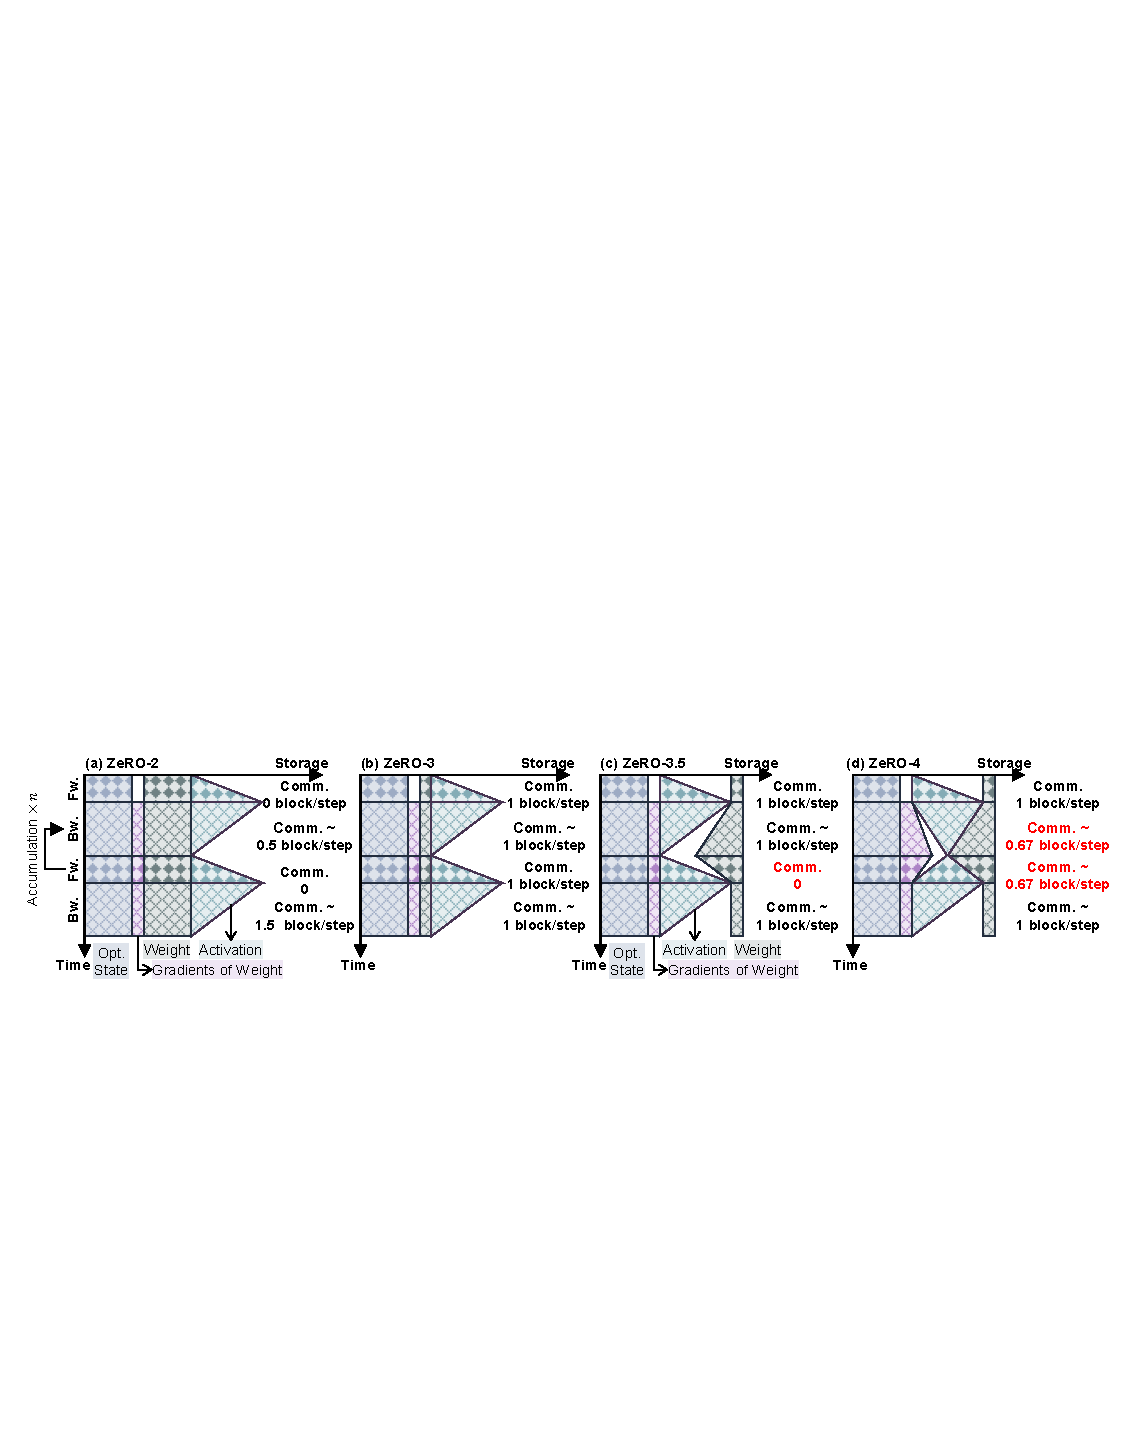
\includegraphics[width=1\linewidth]{figures/FSDP.pdf}
  \caption{Comparison of storage and communication volume during training for ZeRO-2, ZeRO-3 (existing methods), and ZeRO-3.5, ZeRO-4 (proposed by \name{}).}
    \label{fig:FSDP}
\end{figure*}

% 这段感觉应该放到附录，只放图展示结论即可
Figure \ref{fig:FSDP}(a-b) illustrates the approximate changes in storage and communication volume during training for ZeRO-2 and ZeRO-3. Figure \ref{fig:FSDP}(a) illustrates the storage and communication changes in ZeRO-2. During the forward pass, activation storage on each device increases as new activations are generated. In the backward pass, activations are consumed and released. In the final backward step of a batch, each device performs a reduce-scatter of gradients of weights with other devices to update its optimizer state and the corresponding weight shard; old weights can then be discarded. To balance communication load, ZeRO-2 typically performs an all-gather of new weights at the start of the next batch's first forward pass. Assuming each layer's forward computation takes one step and each device transmits one block of data per weight or gradient transfer, the communication volume per device during the first forward is 1 block/step. In the final backward, only gradients of weights are communicated, and since each backward layer takes about twice as long as a forward layer (2 steps), the average communication volume is 0.5 block/step. In practice, multiple gradient accumulation steps are performed; Figure \ref{fig:FSDP} shows only one accumulation, but this process is usually repeated many times and dominates training cost. During accumulation, since ZeRO-2 stores all weights on each device, only the reduce-scatter of weight gradients is needed during backward, with communication volume calculated as 0.5 block/step. ZeRO-3, by sharding the weights, achieves greater memory savings compared to ZeRO-2, as each device only stores a portion of the weights. However, during gradient accumulation, every forward and backward pass for each layer requires an all-gather operation to assemble the complete weights on each device before computation. Consequently, the average communication volume per device for both forward and backward passes is 1 block per step, which becomes the primary performance bottleneck in ZeRO-3. If a strategy could be found that achieves the memory savings of ZeRO-3 while approaching the communication efficiency of ZeRO-2, it would be highly valuable.

\subsection{Dependency and Partial Temporal Order}
\label{sec:dependency}

% 前两句的过度不自然
At this point, the benefits of the data-monistic approach become apparent. To demonstrate this, we present a case study using \name{} (evaluated in Section \ref{sec:exp}), which builds upon ZeRO-3 by introducing additional constraints to enable further optimization. Specifically, during the backward accumulation phase, activations are progressively consumed. Since the memory footprint of activations typically exceeds that of weights, the memory freed from released activations can be repurposed to store incoming weight shards for the current layer. During the next forward pass, these weight shards are discarded layer by layer, and the released memory is used to store newly generated activations. This approach eliminates the need for all-gather communication of weights during the forward accumulation phase. As shown in Figure \ref{fig:FSDP}(c), we refer to this strategy as ZeRO-3.5. 

To implement this, we introduce a new primitive, \texttt{order}. As introduced Section \ref{sec:abstraction}, the set of events associated with a CAT defines its space-time trajectory, while ordering constraints between events specify the temporal sequence of operations during execution (Figure \ref{fig:primitive_intro2}(a)). A typical use of event ordering is to ensure dependency constraints between CATs. For example, consider two CATs, $T_1$ and $T_2$, where the generation of $T_2$ depends on the existence of $T_1$. The corresponding constraint is that the start event of $T_2$ ($T_2\rightarrow\mathrm{start}$) cannot occur before the complete event of $T_1$ ($T_1\rightarrow\mathrm{complete}$). The system implicitly creates events to mark these "complete" and "start" points. The primitive \texttt{order(event1, event2)} explicitly enforces a temporal sequence, ensuring that \texttt{event1} occurs before \texttt{event2} (Figure \ref{fig:primitive_intro2}(b)). For ZeRO-3.5, we use such as \texttt{order($A[i]^{\mathrm{microbatch}+1}\rightarrow\mathrm{complete}$, $W\rightarrow\mathrm{complete}$)} to ensure that the gathered weights during the backward pass are retained until the corresponding activations for the next micro-batch are completed. We can further propose ZeRO-4 that leverages the \texttt{order} primitive to selectively delay all-reduce operations on weight gradients, enabling more balanced forward communication by fully utilizing the variations in available memory capacity (Figure \ref{fig:FSDP}(d)).
% ZeRO-4的叙述有些不太清楚（ZeRO-4还挺复杂的）-> 我觉得基本能get idea，这个太复杂了，而且好处很难说清楚，通信量实际上是一样的，但是通信延迟隐藏更容易了（具体有没有性能提升可能需要实验证明）

It is worth noting that it is impossible to precisely define the physical time of a constraint point in \name{}. Therefore, all temporal coordinates are logical time coordinates based on ordering constraints. For distributed systems, the Lamport timestamp is a highly effective logical clock for this purpose. A Lamport timestamp is a simple counter maintained by each device. It is incremented for each local event, and when a cross dependency is trigger, the device carries the later event updates its clock to the maximum of its own value and the timestamp of the device with the former event, then increments it. This mechanism esures a partial ordering of events across the system. In \name{}, Lamport timestamps are not exposed at the primitive level. Instead, users specify temporal dependencies by defining ordering constraints. The underlying compilation and search systems then automatically manage the Lamport time system to ensure a valid partial order.

\begin{figure}[h]
  \centering
  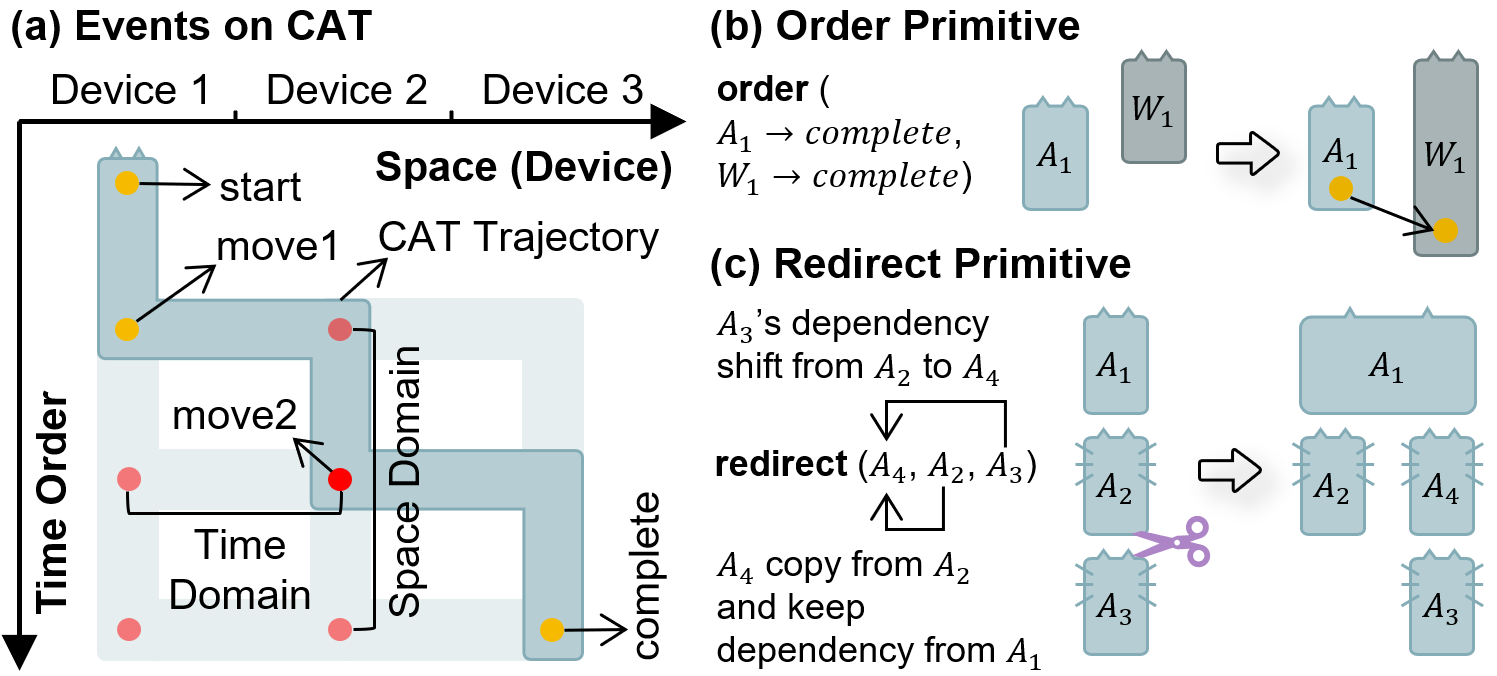
\includegraphics[width=1\linewidth]{figures/primitive_intro2.png}
  \caption{Illustration of dependency management primitives primitives in \name{}. (a) Events control the space-time trajectory of CATs. (b) The \texttt{order} primitive enforces temporal ordering between events. (c) The \texttt{redirect} primitive permutes data dependencies, supporting advanced strategies such as recomputation and dataflow reconfiguration.}
  \label{fig:primitive_intro2}
\end{figure}

For complex dependency operations, we introduce a syntactic sugar primitive: \textbf{\texttt{redirect(tensor1, tensor2, tensor3)}}. This primitive explicitly redirects data dependencies between tensors. As illustrated in Figure \ref{fig:primitive_intro2}(c), if the flow of $A_3$ originally depends on $A_2$, applying the \texttt{redirect} primitive creates $A_4$ from $A_2$ and changes the dependency of $A_3$ from $A_2$ to $A_4$. From a dataflow perspective, the production of $A_3$ initially depends on the completion of $A_2$; after redirection, it depends on $A_4$.

% 附录中增加具体的例子
A key optimization enabled by the \texttt{redirect} primitive is recomputation, also known as activation checkpointing. This technique trades additional computation for reduced memory usage by selectively discarding intermediate activations during the forward pass and recomputing them later when required for the backward pass. Capturing such dynamic changes in data dependencies is challenging for operator-centric frameworks~\cite{lin2024nnscaler}. In contrast, the \texttt{redirect} primitive provides a direct and flexible mechanism to express recomputation. For example, consider a scenario where we want to recompute the activation $A_2$ during the backward pass while keep $A_1$ during forward. By applying \texttt{redirect($A_2$, $A_4$, $A_3$)}, we create a new tensor $A_4$ by recomputing from $A_1$, and update the dependency of $A_3$ that needs to be used in the backward pass to depend on $A_4$ instead of the original $A_2$.

For complex dependency operations, we introduce a syntactic sugar primitive: \textbf{\texttt{redirect(tensor1, tensor2, tensor3)}}. This primitive explicitly redirects data dependencies between tensors. As illustrated in Figure \ref{fig:primitive_intro2}(c), if the flow of $A_3$ originally depends on $A_2$, applying the \texttt{redirect} primitive creates $A_4$ from $A_2$ and changes the dependency of $A_3$ from $A_2$ to $A_4$. From a dataflow perspective, the production of $A_3$ initially depends on the completion of $A_2$; after redirection, it depends on $A_4$. A key optimization enabled by the \texttt{redirect} primitive is recomputation, also known as activation checkpointing. This technique trades computation for memory by discarding intermediate activations during the forward pass and recomputing them for the backward pass. While challenging for operator-centric frameworks to express this dynamic dependency change, our data-centric approach handles it through manipulate of dependencies. 

Let's illustrate with a simple model segment: $A_1 = \text{Layer1}(\text{Input})$, followed by $A_2 = \text{Layer2}(A_1)$. During the backward pass, computing the gradient for Layer2 requires its input, $A_1$. Here is how recomputation is implemented:
\begin{enumerate}
    \item \textbf{Forward Pass}: We compute $A_1 = \text{Layer1}(\text{Input})$ and designate it as a checkpoint. Then, we compute $A_2 = \text{Layer2}(A_1)$. To save memory, we can immediately discard $A_2$ after its use, keeping only the checkpointed $A_1$.
    \item \textbf{Backward Pass Trigger}: When the backward pass needs to compute the gradient for Layer2, it discovers that its required input, $A_2$, is missing.
    \item \textbf{Recomputation and Redirection}: The framework intercepts this dependency request. It re-runs the forward computation from the last checkpoint: $A_4 = \text{Layer2}(A_1)$. This new tensor, $A_4$, holds the same value as the original $A_2$.
    \item \textbf{Dependency Update}: The \texttt{redirect($A_2$, $A_4$, Grad\_Layer2)} primitive is then invoked. This command informs the system that any operation that previously depended on the original (and now deleted) $A_2$—in this case, the gradient calculation for Layer2 (Grad\_Layer2)—should now source its input from the newly computed $A_4$.
\end{enumerate}

In essence, \texttt{redirect} dynamically rewires the data dependency graph, allowing the backward pass to proceed seamlessly with the recomputed activation. This provides a direct and flexible mechanism to implement recomputation without altering the fundamental logic of the backward pass itself.

\subsection{Strategy Space Delineation}

As the preceding discussion shows, \name{}'s primitives are fundamentally a series of declarative constraints. In the absence of any user-defined primitives, the strategy space encompasses the universal set of all valid parallelization plans for a given computation graph and hardware system, constrained only by the inherent data dependencies. The process of applying primitives is not an imperative one that directly modifies a state or carries out an operation; rather, each primitive declaratively refines the strategy space by adding constraints that narrow the universe of possible plans. Once specified, this refined space is handed to a search algorithm (Section \ref{sec:search}) and compilation process (Section \ref{sec:implementation}) to instantiate a concrete, high-performance plan. Consequently, \name{} must also provide mechanisms to help users effectively delineate the strategy space and express preferences for certain types of strategies.

One of the mechanisms is \textbf{domain}. A \textbf{domain} is an iterable set that can represent the range of possible values for time, space, or other parameters. For example, \texttt{d = Domain(Device1 to Device3)} defines the domain as devices 1, 2, and 3. If we write \texttt{assign(tensor, d)}, it means that within the strategy space, the tensor can be assigned to any of these three devices. The light blue region in Figure \ref{fig:primitive_intro2}(a) illustrates the possible CAT trajectory space defined by the space-time domain of event points on CATs. With this mechanism, the element of constraint vector could not be a precise point, but a domain of space-time coordinates.

% 说不清楚，所以leave it for future work
Another mechanism for more advanced space delineation is a \textbf{hole}. Sometimes, while users may not know the exact form of the scheduling strategy for certain CATs and hope the search algorithm can find unexpected strategies, they still have a preference for the types of scheduling operations to be applied. Such structural preferences in a sub-strategy space can be expressed by a \texttt{hole(tensors, grammar)} primitive. Its purpose is to generate a structural variable—a "hole"—and bind it to a potential scheduling grammar, for example \texttt{split(tensor, Domain(1 to 4))}, providing a set of scheduling options for the search algorithm. Although the hole mechanism allows users to delineate the strategy space more precisely, it is not a core focus of the current version of \name{}. And considering the implementation complexity of the "grammar", we leave it for future work.

\section{Constraint-Based Potential Descent Search}
\label{sec:search}

The primary challenge in distributed training is not merely tuning parameters but performing true strategy search—discovering a high-performance parallelization plan from various vast and complex strategy spaces. Most existing frameworks operate by first defining a fixed strategy template, such as 3D parallelism or a template crafted by domain-specific primitives, and then conducting a parameter search within that template to determine variables like partition sizes or device mappings. This fundamentally limits the search to human-predefined designs. In contrast, our goal is to enable the search for diverse and even novel strategies that emerge from a space that contains unforeseen possibilities. Any strategy satisfying the space's constraints defined by \name{}'s primitives can be discovered, moving beyond parameter tuning to strategy-level exploration.

However, genuine strategy-level exploration remains highly challenging due to the heterogeneous and combinatorial nature of operator-based search spaces. A parallelization strategy is determined by a complex interplay of fundamentally distinct decisions: how to partition tensors (e.g., data or tensor parallelism), where to place computations, when to schedule operations, and whether to recompute data or retrieve it from remote memory. This results in a fragmented and rugged search landscape, where even minor changes in one decision dimension—such as switching from recomputation to data fetching—can yield drastically different and structurally incomparable solutions. As a result, traditional search algorithms cannot employ unified optimization techniques (such as descent methods) and must instead rely on intricate, hand-crafted heuristics to traverse a space composed of discrete, non-interchangeable choices. This complexity renders the systematic discovery of novel strategies intractable.

\begin{algorithm}[h]
\caption{Structured Local Search for Strategy Discovery}
\label{alg:structured_search}
\begin{algorithmic}[1]
\STATE \# Input: Initial parallelization plan $S_{initial}$
\STATE \# Output: Optimized parallelization plan $S_{final}$
\STATE $S_{current} \gets S_{initial}$
\STATE $P_{current} \gets \text{CalculatePotential}(S_{current})$
\FOR{$i = 1$ to $max\_iterations$}
  \STATE $improved \gets \text{false}$
  \STATE $M_{candidates} \gets \text{GetCandidateMoves}(S_{current})$
  \FOR{each move $m$ in $M_{candidates}$}
    \STATE $S_{neighbor} \gets \text{ApplyMove}(S_{current}, m)$
    \STATE $P_{neighbor} \gets \text{CalculatePotential}(S_{neighbor})$
    \IF{$P_{neighbor} < P_{current}$}
      \STATE $S_{current} \gets S_{neighbor}$
      \STATE $P_{current} \gets P_{neighbor}$
      \STATE $improved \gets \text{true}$
      \STATE \textbf{break} \# First-improvement strategy
    \ENDIF
  \ENDFOR
  \IF{not $improved$}
    \STATE \textbf{break} \# Local minimum reached
  \ENDIF
\ENDFOR
\STATE \textbf{return} $S_{current}$
\end{algorithmic}
\end{algorithm}



Our data-monistic abstraction is suited to address this complex strategy search problem by enhancing the "searchability" of the solution space. A mathematical analysis is beyond the scope of this paper, but we highlight two key properties that provide important intuition. First, it establishes \textbf{Topological Homogeneity and Continuity}. Unlike operator-based abstractions which yield a discrete space of strategies, our approach creates a continuous, connected landscape. In this space, canonical strategies (e.g., DP, TP) are not isolated points but interconnected sub-regions. A transition between them, such as from pure Data Parallelism to a hybrid FSDP-like strategy, can be realized as a traversable path of incremental changes—for instance, by progressively sharding one tensor at a time. This continuity makes the space amenable to systematic exploration via local search or gradient-based methods. Second, it provides \textbf{Fine-Grained Decision Space}: The abstraction provides a higher-resolution search space by defining constraints on fine-grained data states (individual tensors at specific time-points) rather than on coarse-grained operators. This transforms a single, high-stakes decision (e.g., "apply FSDP to this entire block?") into numerous, low-stakes decisions (e.g., "shard tensor A?", "prefetch tensor B?"). For a greedy search algorithm, this granularity is critical: a sub-optimal local choice on a single tensor is less likely to derail the entire search trajectory, offering more opportunities for subsequent steps to compensate and navigate away from poor local optima.


% First, it establishes \textbf{Topological Homogeneity and Continuity}. Operator-based abstractions are typically composed of discrete and qualitatively different operation types. By representing any strategy as a unification of CATs, transitions between vastly different high-level strategies can be decomposed into a sequence of small, incremental modifications to the underlying CAT abstraction. This creates a connected and high-resolution landscape where strategies are not isolated points but interconnected neighbors, making the space far more amenable to systematic exploration by local search algorithms. Second, it provides \textbf{Heuristic Consistency}. By defining scheduling fine-grained constraints on CATs rather than coarse-grained operators, the abstraction increases the number of decision variables (More tensors than operators, and a tensor could have many event points). Although the complexity of strategy expression has been increased, the higher-dimensional space creates more "escape routes" from local optima, enabling more consistent and reliable greedy search paths. Together, these properties transform the intractable problem of strategy discovery into a structured and tractable optimization task.

Building upon these properties, we propose a scheduling model inspired by potential field methods, which transforms the scheduling problem into a search for the minimum energy state within a multi-dimensional potential field. The search process manifests as modifications to CATs' constraint vector, which include: (1) specifying concrete space-time intervals, (2) altering the vector's dimensionality by adding or removing event points, and (3) generating new constraint vectors for newly created CATs.

For any given parallel plan, we define a system-wide "potential energy". This energy is evaluated based on the "pressure" on each device, where high pressure corresponds to resource oversubscription (e.g., exceeding memory capacity) or poor performance. Our heuristic search algorithm then guides each modification to a CAT's constraint vector in the direction that yields the steepest descent in the overall potential energy. To offer an intuitive analogy, one can imagine the "pressure" on each device as the "water level" at different locations in a pond. Each CAT acts as an independent stream of water, naturally flowing from high-pressure regions to low-pressure ones, thereby lowering the system's overall potential energy.

To formalize this search process, we employ a structured local search algorithm guided by the principle of potential energy minimization. The algorithm iteratively refines a parallelization plan by exploring neighboring solutions and accepting modifications that reduce the system's overall potential. Algorithm \ref{alg:structured_search} presents the pseudocode for this algorithm.

The algorithm operates as follows. It begins with an initial parallelization plan randomly selected from the strategy space, $S_{initial}$. The algorithm then enters an iterative loop that seeks to find a better plan at each step. The \texttt{CalculatePotential} evaluates the global potential of a given plan $S$, acting as the objective function. This value quantifies the plan's inefficiency and the extent of resource oversubscription. A lower potential signifies a more balanced and efficient plan. In each iteration, the \texttt{GetCandidateMoves} heuristically generates a list of promising modifications. Instead of exploring all possible moves, it focuses on "problem areas". For example, it identifies devices with high potential (e.g., memory overflow) and proposes moves for the CATs on those devices, such as migrating a CAT to a less loaded device (\texttt{move}) or breaking a large CAT into smaller ones (\texttt{split}). The algorithm then iterates through these candidate moves, applies each one to generate a neighbor plan using \texttt{ApplyMove}, and evaluates its potential. Following a first-improvement strategy, it immediately accepts the first move that results in a lower potential, updates the current plan, and restarts the iteration. If no candidate move yields an improvement, the algorithm concludes that it has reached a local minimum and terminates.

There are numerous implementation details in the search algorithm. For instance, the \texttt{GetCandidateMoves} function operates in two stages: it first examines the optimal moves for each event point in the constraint vector of a CAT, and then combines these local moves into an overall modification of the constraint vector. Furthermore, after a specific change to a constraint vector is applied, the \texttt{CalculatePotential} function evaluates not only global metrics such as memory pressure or overall computation latency, but also the pressure to satisfy inter-constraints among CATs (e.g., the requirement to reach a certain device before a particular event for computation). These details, as well as heuristic choices made during the search process (such as preferring not to release a CAT when sufficient memory is available), can lead to different strategy outcomes. Due to space limitations, we provide further discussion of these details in Appendix \ref{sec:search_details}.


\section{Implementation}
\label{sec:implementation}

% because it builds on the explicit scheduling of data trajectories
The data-monistic abstraction of \name{} represents a fundamental shift from existing operator-centric distributed training frameworks like DeepSpeed or Megatron, whose core architectures (IR, schedulers, runtimes) are deeply integrated to schedule operators. Retrofitting \name{} into these frameworks is extremely difficult. Moreover, this architectural mismatch culminates in an incompatible runtime. While existing systems are designed to execute a pre-compiled sequence of computational kernels and communication collectives, it remains an open research topic how to dynamically interpret a data-centric schedule to generate efficient low-level CUDA kernels on the fly. Therefore, \name{} is not implemented as an end-to-end system but rather serves as a strategy exploration framework. It discovers parallelization plans that are then manually implemented for high-performance execution.

Besides the above the difficulties, this work mainly focus on three main challenges in implementing \name{}. First, the realization of constraint-declarative primitives in high-level languages and the corresponding abstraction in the intermediate representation (IR). Second, the formulation and solving of the constrained optimization problem (COP) underlying our proposed search algorithm. Third, the compilation of the strategy space, which automates certain data constraint processes to avoid tedious manual implementation. The basic implementation stack of \name{} is shown in Figure \ref{fig:implementation}.

\begin{figure}[h]
  \centering
  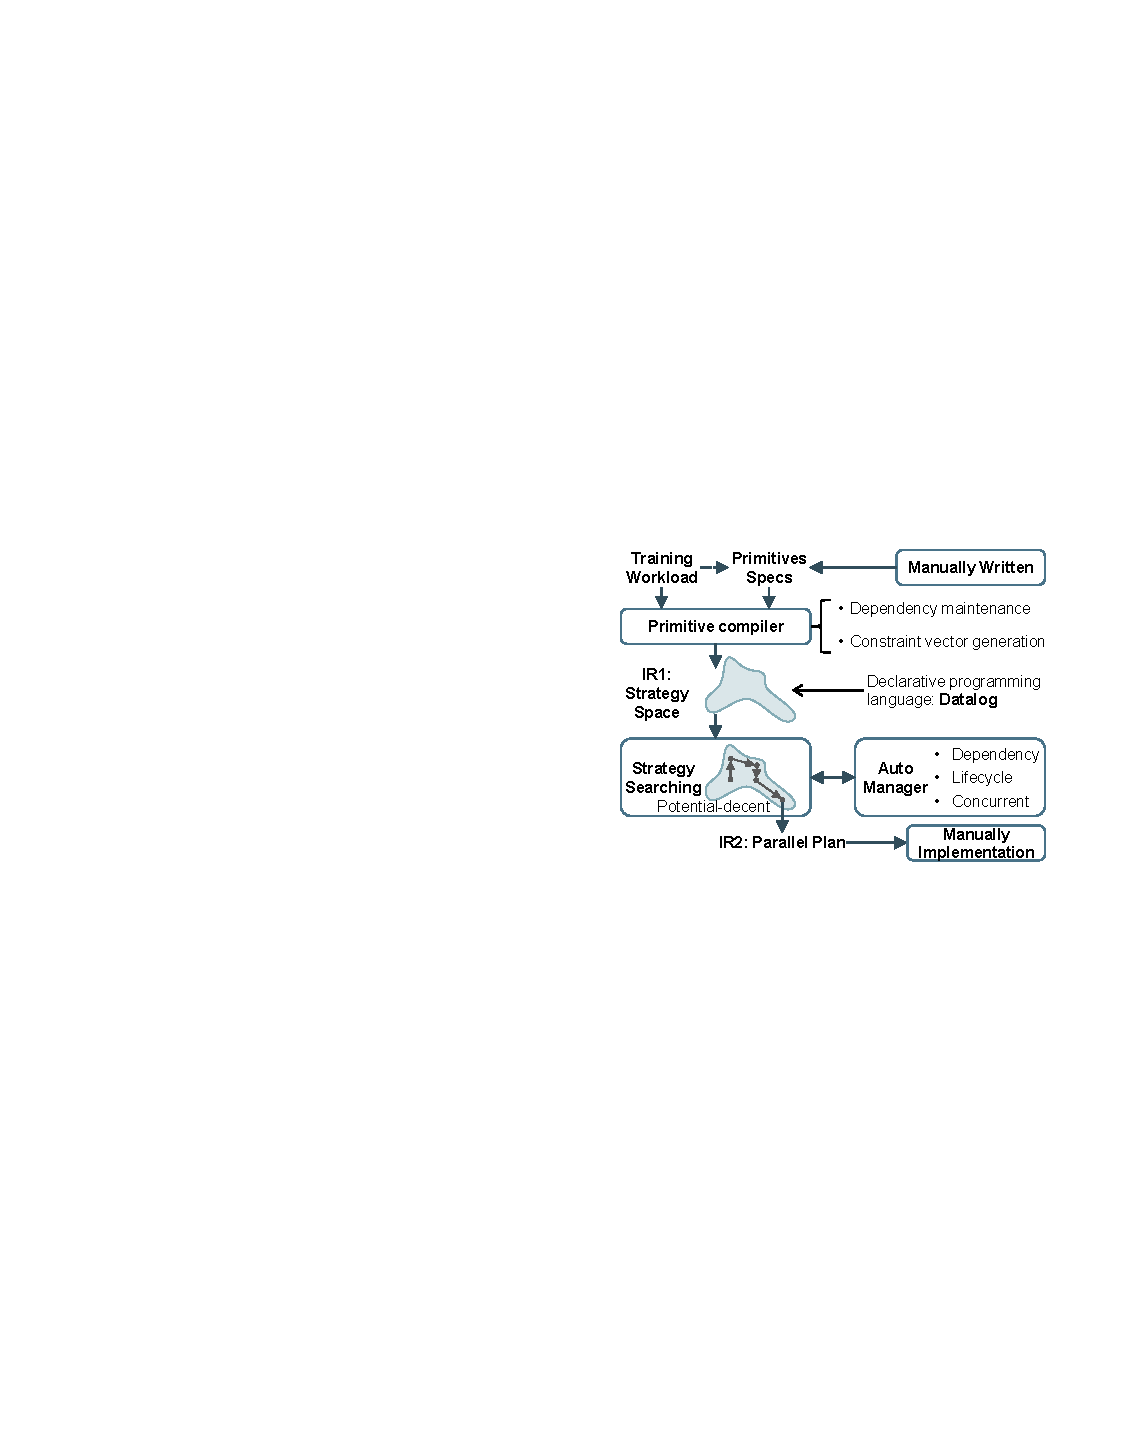
\includegraphics[width=0.83\linewidth]{figures/implementation.pdf}
  \caption{Implementation stack of \name{}.}
    \label{fig:implementation}
\end{figure}

\textbf{Primitive and IR Realization.} The primitives are implemented using Datalog, a declarative programming language, which provides a Python interface. The Datalog rules that describe the primitives and their constraints are translated into a COP formulation in Google OR-Tools, which serves as the backend for the subsequent search and compilation stages.

\textbf{Strategy Search with COP Engine.} The strategy search is conducted using the potential descent algorithm detailed in Section \ref{sec:search}. This process is augmented with constraint propagation, which dynamically prunes the search space during constraint challenging. The constraint propagation is handled by the Google OR-Tools solver, which maintains consistency and reduces the set of feasible solutions as the search progresses.

\textbf{Auto-Solving Compiler.} A compiler component automates several aspects of schedule generation. For dependency management, it establishes connections between CATs, manages the Lamport logical time system, and resolves data dependencies by identifying the nearest available data block. For lifecycle management, it tracks the usage of each CAT and inserts release operations for tensors with no further downstream dependencies. For concurrency management, it handles concurrent events within the logical clock system, enabling optimizations like computation-communication overlap.

More implementation details are provided in Appendix \ref{sec:implementation_details}.

\section{Evaluation}
\label{sec:exp}

Kindly ask the reviewers to give their evaluation.

\section{Related Work}

\section{Conclusion}

In this paper, we present \name{}, a data-monistic abstraction for distributed training that unifies the representation of data and computation. By introducing the concept of Constraint-Aware Tensors (CATs) and a set of data-centric primitives, \name{} enables the declarative specification of complex parallelization strategy spaces. We also propose a constraint-based potential descent search algorithm that systematically explores this vast strategy space, discovering efficient parallelization plans that outperform existing methods. However, \name{} focuses on high-level distributed scheduling and does not extend to micro-architectural optimizations tightly coupled with hardware, such as PagedAttention. Furthermore, this paradigm shift introduces significant implementation challenges, and a full end-to-end system remains an area for future work. In addition, more efficient search algorithms, especially for runtime scheduling, could be further explored.


%-------------------------------------------------------------------------------
\bibliographystyle{plain}
\bibliography{ref.bib}

\appendix

\section{Data-Centric Primitives in \name{}}
\label{sec:all_primitives}

\begin{table*}[h]
\centering
\resizebox{\textwidth}{!}{%
\begin{tabular}{p{0.4\textwidth}p{0.6\textwidth}}
\toprule
Primitives                             & Usage \\ \midrule
\texttt{split(tensor, split\_vector, split\_tensors)}         & \texttt{tensor} represents the tensor to be partitioned. \texttt{split\_vector} represents the vector guiding how to partition \texttt{tensor}. \texttt{split\_tensors} are the result tensors. \\
\texttt{assign(tensor, device)}        & Assign \texttt{tensor} to \texttt{device}. \\
\texttt{copy(src\_tensor, device, dst\_tensor, path)} & Copy \texttt{src\_tensor} from its current device to \texttt{device}. The copied tensor on \texttt{device} can be accessed through the pointer \texttt{dst\_tensor}. \texttt{path} represents the copy path. \\
\texttt{cut(src\_tensor, device, dst\_tensor, path)} & Cut \texttt{src\_tensor} from its current device to \texttt{device}. The moved tensor on \texttt{device} can be accessed through the pointer \texttt{dst\_tensor}. \texttt{path} represents the cut path. After cut, \texttt{src\_tensor} will be freed from memory.        \\
\texttt{reduce(src\_tensors, device, dst\_tensor, path)} & Reduce \texttt{src\_tensors} into \texttt{dst\_tensor}. The reduction result will be placed on \texttt{device}. \texttt{path} represents the reduction path.     \\
\texttt{redirect(tensor1, tensor2, tensor3)} & Redirect the data dependencies between \texttt{tensor1} \& \texttt{tensor3} to \texttt{tensor2} \& \texttt{tensor3}.                                        \\
\texttt{order(event1, event2)}        & Enforce temporal order between \texttt{event1} and \texttt{event2}.  \texttt{event1} executes before \texttt{event2}.                                                                                      \\ \bottomrule
\end{tabular}%
}
\caption{Data-centric primitives for parallelization space construction in \name{}.}
\label{tab:primitives}
\end{table*}

\section{Details of ZoRO strategies}

FSDP is a widely-adopted data parallelism strategy that coordinates computation and data movement. It shards model parameters, gradients, and optimizer states across devices to reduce memory. During training, each device holds only a shard of the weights. For a forward pass, a device gathers the full parameters for the current layer, performs the computation, and then discards the full parameters, keeping only its shard. For the backward pass, gradients are computed locally and then reduced and sharded directly to the target devices using a reduce-scatter operation, avoiding redundant storage. This sharding strategy is often described in levels, inspired by the ZeRO (Zero Redundancy Optimizer) framework~\cite{rajbhandari2020zero}. ZeRO-1 shards optimizer states, ZeRO-2 adds gradient sharding, and ZeRO-3 (the typical FSDP implementation) shards parameters as well for maximum memory savings. Algorithm \ref{alg:fsdp} shows how \name{}'s primitives can represent the core of ZeRO-2/3. 

Figure \ref{fig:FSDP}(a-b) illustrates the approximate changes in storage and communication volume during training for ZeRO-2 and ZeRO-3. Figure \ref{fig:FSDP}(a) illustrates the storage and communication changes in ZeRO-2. During the forward pass, activation storage on each device increases as new activations are generated. In the backward pass, activations are consumed and released. In the final backward step of a batch, each device performs a reduce-scatter of gradients of weights with other devices to update its optimizer state and the corresponding weight shard; old weights can then be discarded. To balance communication load, ZeRO-2 typically performs an all-gather of new weights at the start of the next batch's first forward pass. Assuming each layer's forward computation takes one step and each device transmits one block of data per weight or gradient transfer, the communication volume per device during the first forward is 1 block/step. In the final backward, only gradients of weights are communicated, and since each backward layer takes about twice as long as a forward layer (2 steps), the average communication volume is 0.5 block/step. In practice, multiple gradient accumulation steps are performed; Figure \ref{fig:FSDP} shows only one accumulation, but this process is usually repeated many times and dominates training cost. During accumulation, since ZeRO-2 stores all weights on each device, only the reduce-scatter of weight gradients is needed during backward, with communication volume calculated as 0.5 block/step. ZeRO-3, by sharding the weights, achieves greater memory savings compared to ZeRO-2, as each device only stores a portion of the weights. However, during gradient accumulation, every forward and backward pass for each layer requires an all-gather operation to assemble the complete weights on each device before computation. Consequently, the average communication volume per device for both forward and backward passes is 1 block per step, which becomes the primary performance bottleneck in ZeRO-3. If a strategy could be found that achieves the memory savings of ZeRO-3 while approaching the communication efficiency of ZeRO-2, it would be highly valuable.

\section{Details and Concerns About Search Algorithm}
\label{sec:search_details}

1. Symmetry Constraints: To improve search efficiency and reduce highly irregular solutions, symmetry constraints can be introduced into the search algorithm. That is, CATs with symmetric constraint vectors are treated as equivalent, and their scheduling actions are bound together during the search process.

2. Collectivity and Individuality of Potential: In the main text, we describe the calculation of potential as a global property, implying that the potential landscape is identical for each CAT. However, this is not strictly the case. Some metrics that influence "potential," such as memory pressure or overall computation latency, are indeed global. However, each CAT may also be subject to individualized constraints that exert personalized pressure, such as the requirement to arrive at a specific device before a certain event to synchronize with another CAT. As the event approaches, the pressure for the CAT to flow toward that device increases. Therefore, the movement of each CAT is not determined solely by the global potential.

3. In the absence of the hole mechanism described in the main text, it is not possible to constrain non-domain strategy spaces. Thus, by default, our search algorithm allows free exploration of these strategy spaces.

4. The search algorithm should be guided by certain heuristics. For example, in the absence of pressure-driven guidance, a CAT may simply remain on its current device without being released. Such heuristics can help the algorithm discover anticipated strategy optimization directions.

5. Two-level Heuristic Descent: In theory, it is possible to treat the constraint vector of a CAT as a whole and perform heuristic descent on it. However, finding the optimal descent direction would require enumerating all possible next-step transformations of the constraint vector, which is computationally infeasible due to the combinatorial explosion when multiple event points are involved. To address this, we adopt a two-level heuristic descent approach. At the first level, we perform local heuristic descent for each event point, identifying the optimal descent direction for each (i.e., applying a coordinate descent algorithm to the constraint vector). At the second level, we combine these locally optimal descent directions to determine the overall optimal descent direction for the entire constraint vector.

6. It is not accurate to state that the search process continuously refines the strategy space, as the potential descent algorithm merely iterates from one strategy solution to another without altering the strategy space itself. However, it is correct to say that the process of writing primitives refines the strategy space. In addition, a refinement engine exists within the search algorithm—using techniques such as constraint propagation—to prune the strategy space.

\section{Implementation Details}
\label{sec:implementation_details}

%%%%%%%%%%%%%%%%%%%%%%%%%%%%%%%%%%%%%%%%%%%%%%%%%%%%%%%%%%%%%%%%%%%%%%%%%%%%%%%%
\end{document}
%%%%%%%%%%%%%%%%%%%%%%%%%%%%%%%%%%%%%%%%%%%%%%%%%%%%%%%%%%%%%%%%%%%%%%%%%%%%%%%%

%%  LocalWords:  endnotes includegraphics fread ptr nobj noindent
%%  LocalWords:  pdflatex acks
